
\section{Analyzing Post-Deletion Agent Behavior}
\label{sec:tech_analysis}
%
To investigate how commercial LLM agents respond to data deletion requests and whether previously disclosed information remains retrievable afterward (RQ3), we developed a new Data Injection-Deletion-Recall (DIDR) analysis pipeline.
%
We also compare observed agent behavior with users' deletion expectations (RQ4).
%
This section describes our methodology and presents the findings for RQ3 and RQ4.

\subsection{Post-Deletion Analysis Methodology}
%
Our methodology consists of three components: (1) the DIDR pipeline, which conducts controlled experiments across LLM agents and deletion methods using traceable synthetic facts; (2) outcome measures and analysis procedures for evaluating post-deletion agent behavior; and (3) comparisons between observed agent behavior and users' deletion expectations and verification strategies.
%
We describe each component in detail below.

\subsubsection{DIDR Analysis Pipeline}
%
\label{sec:didr}
%
As illustrated in Figure~\ref{fig:didr}, the DIDR pipeline comprises three stages: \textit{data injection}, which introduces a synthetic fact into an LLM agent; \textit{data deletion}, which applies a deletion method; and \textit{data recall}, which examines whether the injected fact remains retrievable afterward.
%
Each test case combines a synthetic fact, an injection method, a deletion method, and an LLM agent.
%
By injecting synthetic facts with unique values, we can attribute subsequent recall of those values to information introduced during our experiments.
%
The pipeline supports two complementary experimental approaches.
%
\textit{UI-action experiments} examine the information-entry and deletion controls available through each agent's interface, whereas \textit{prompt-based experiments} evaluate deletion requests authored by participants in our user study (Section~\ref{sec:user_study}).
%
In both approaches, deletion occurs at least 48 hours after injection, and recall testing occurs at least 30 days after deletion.
%
We chose this interval because several LLM agents (e.g., XX~\cite{}, XX~\cite{}, and XX~\cite{}) document that deleted data may remain in their systems for up to 30 days, and we applied the same interval across all agents for consistency.
%
We use Playwright-based automation~\cite{} for supported interactions and conduct the remaining operations manually.

\begin{figure*}[t]
    \centering
    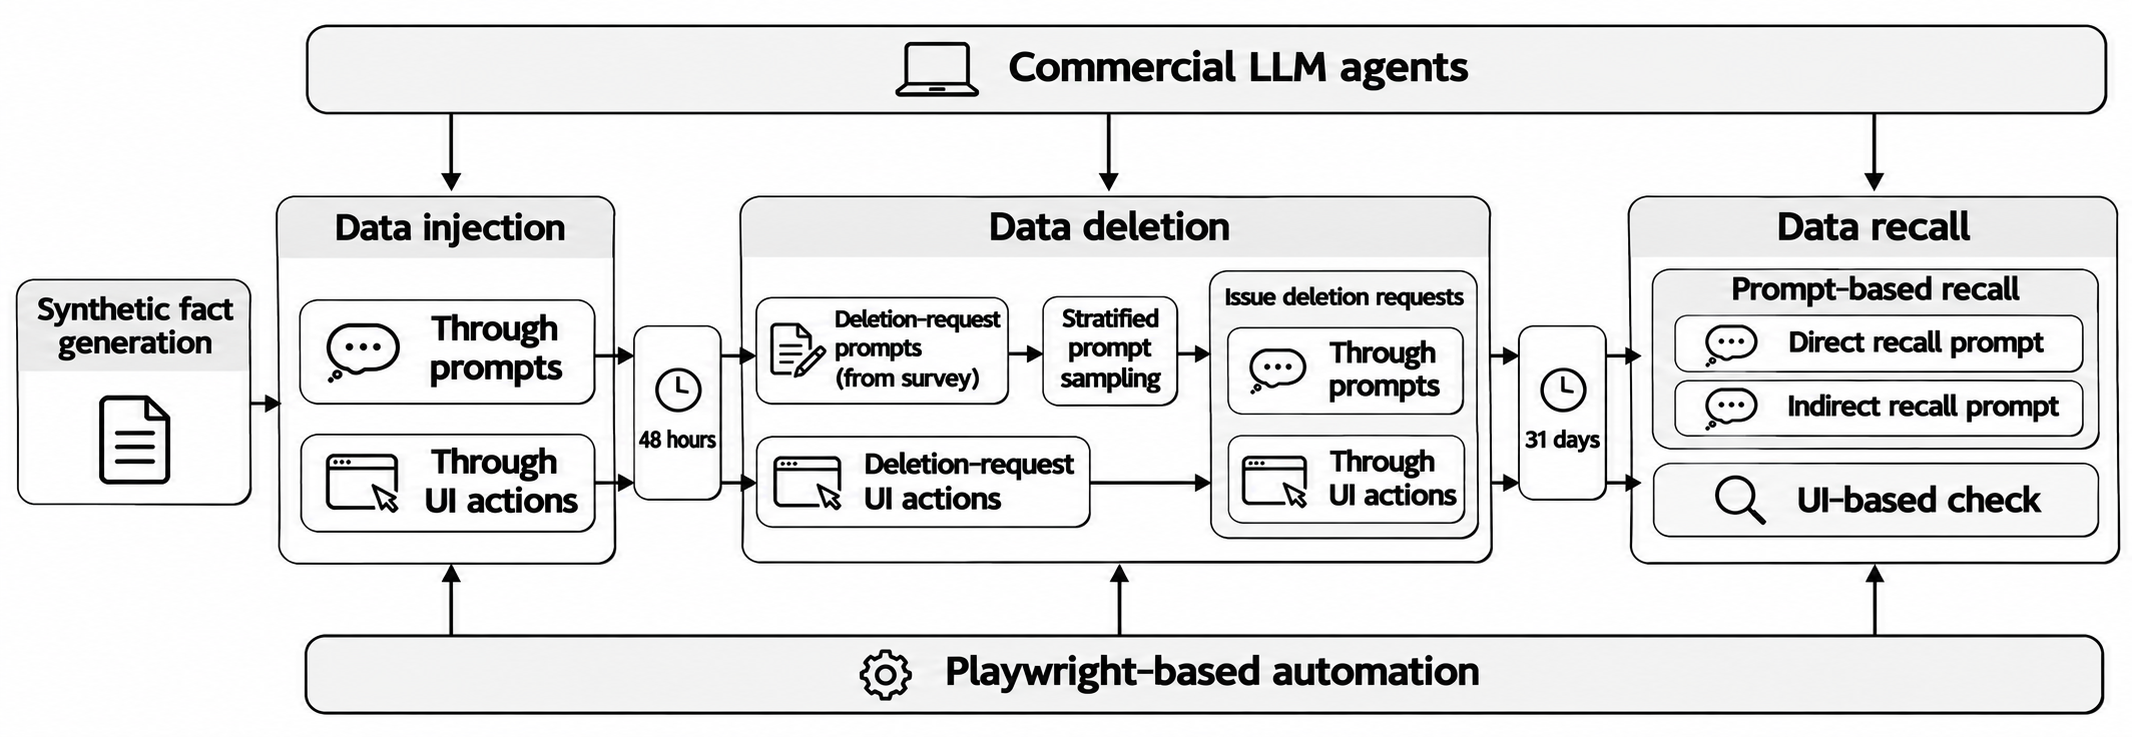
\includegraphics[width=\textwidth]{figures/DIDR.png}
    \caption{Overview of the DIDR analysis pipeline. Synthetic facts are injected into commercial LLM agents through prompts or UI actions, followed by deletion at least 48 hours later and recall testing at least 30 days after deletion. Deletion is performed using available agent controls or participant-authored deletion-request prompts, while recall is assessed through direct and indirect prompts and UI-based checks. Playwright automates supported interactions, with other operations performed manually.}
    \label{fig:didr}
\end{figure*}

\para{Synthetic fact generation}
%
To trace subsequent recall to a specific injected fact, we generated synthetic facts unlikely to have been previously encountered by LLM agents.
%
Each fact is represented as an $\langle$ \texttt{entity}, \texttt{attribute}, \texttt{value} $\rangle$ tuple, where the \texttt{entity} represents an everyday object or project, the \texttt{attribute} identifies a property, and the \texttt{value} is a unique synthetic code name comprising two to four words.
%
For example, one fact is $\langle$\textit{a scarf I'm knitting}, \textit{name}, ``\textit{Magnifier King Broom}''$\rangle$.
%
Following the canary-based approach of Carlini et al.~\cite{carlini2019secret}, each value is unique to one test case, allowing us to trace subsequent retrieval of the value to its corresponding injection.
%
We manually curated entities representing everyday objects and projects.
%
Values were generated using the EFF long word list~\cite{}, retaining words with a noun sense in WordNet~\cite{} while excluding terms associated with weapons, drugs, sexual content, and other potentially sensitive categories.
%
This filtering reduced the possibility that platform safety restrictions would interfere with recall observations.
%
Each fact was embedded in a casual conversational sentence, with wording varied across test cases to resemble ordinary user interactions.

\para{Data injection}
%
We injected synthetic facts through the \textit{information-entry} mechanisms supported by each LLM agent.
%
For UI-action experiments, we systematically examined each agent's web interface to identify available mechanisms, following an approach similar to prior walkthroughs of LLM privacy controls~\cite{li2026privacy}.
%
These mechanisms included \textit{casually disclosing information during a conversation}, \textit{explicitly requesting the agent to remember information}, and \textit{entering information through dedicated interfaces}, such as saved-memory pages~\cite{}, custom instructions~\cite{}, or saved-information pages~\cite{}.
%
We tested only the mechanisms available for each agent.
%
For prompt-based experiments, we held the injection method constant by introducing each fact as a casual statement in a conversation, allowing us to examine different deletion requests without varying how the information was initially disclosed.
%
In both approaches, we waited at least 48 hours before initiating deletion to allow time for the agent to process and potentially retain the injected information.

\para{Data deletion}
%
We evaluated deletion through two complementary approaches.
%
For UI-action experiments, we applied the deletion methods identified in our interface walkthrough (Table~\ref{tab:methods}), including UI-based controls targeting conversations, saved memories, and account-level data management.
%
This approach also included 13 test cases in which deletion was requested through a conversational prompt.
%
For each agent, we further tested its most extensive available deletion procedure by combining all applicable controls.
%
We excluded two methods included in the survey: \textit{deleting the account}, which would prevent subsequent observation of the same account, and \textit{filing a request with the company}, which is handled outside the agent.
%
Across the six agents, we designed 73 UI-action test cases and executed 67, as the remaining six required paid Perplexity features.
%
To prevent interference between test cases, we used dedicated accounts for deletion procedures that could affect other stored information.
%
Where multiple deletion procedures shared an account, we executed them from narrower to broader scopes (e.g., deleting a single conversation before clearing all conversation history) to avoid prematurely removing facts associated with other test cases.

For prompt-based experiments, we used deletion requests authored by survey participants to reflect how users express deletion intentions in natural language (i.e., participant-authored deletion-request prompts in Section~\ref{subsubsec:questions}).
%
In total, 209 participants provided 415 requests, including participants without prior deletion experience, as the prompt-writing task was hypothetical.
%
After removing duplicate and repeated requests, 375 distinct requests remained, and identifying information was redacted from seven requests.
%
Testing all 375 requests across six agents would have required 2,250 test cases under free-tier usage constraints.
%
Therefore, we grouped the requests into seven keyword-based categories according to references to deletion targets, such as memories, conversations, accounts, or databases, and selected 138 requests through stratified random sampling.
%
We selected at least 15 requests per category and included all requests from the two smallest categories to ensure coverage of less frequent formulations.


To characterize the selected requests, two researchers independently coded the 138 requests along seven dimensions: \textit{deletion location}, \textit{justification}, \textit{data named}, \textit{mood}, \textit{tone}, \textit{verb}, and \textit{accompanying request}.
%
They initially coded a subset of 50 requests independently without a shared codebook, reconciled their identified dimensions into a common codebook, and refined it through additional independent coding rounds.
%
They then independently coded all 138 requests and resolved disagreements through discussion.
%
Inter-rater agreement was high, with a pooled Gwet's AC1~\cite{gwet2008ac1} of 0.954 across the seven dimensions and at least 0.89 for each dimension (Table~\ref{tab:coding}).
%
The reconciled codes were subsequently used to examine associations between deletion-request wording and recall outcomes.


Five sampled requests asked agents to delete all user data and were excluded because they could interfere with other test cases.
%
We submitted the remaining 133 requests to all six agents, yielding 798 prompt-based test cases.
%
Together with the 67 executable UI-action test cases, our main evaluation comprised 865 test cases.
%
We separately designed 12 supplemental test cases involving uploaded files, examining conversation deletion and each agent's most extensive deletion procedure.
%
Eleven were executable, while the remaining case required a paid Perplexity feature.
%
These supplemental cases were analyzed separately because uploaded content may be accessible through the conversation context, saved memories, or both.

\begin{table}[t]
\centering
\caption{Inter-rater agreement for coding 138 participant-authored deletion requests. AC1 denotes Gwet's agreement coefficient.}
\label{tab:coding}
\small
\begin{tabular}{@{}lrrr@{}}
\toprule
Dimension & Agreed & \% & AC1 \\
\midrule
Deletion location & 125/138 & 90.6 & 0.890 \\
Justification & 131/138 & 94.9 & 0.943 \\
Data named & 133/138 & 96.4 & 0.956 \\
Mood & 133/138 & 96.4 & 0.959 \\
Tone & 137/138 & 99.3 & 0.990 \\
Verb & 131/138 & 94.9 & 0.947 \\
Accompanying request & 133/138 & 96.4 & 0.962 \\
\midrule
All dimensions (966 ratings) & 923/966 & 95.5 & 0.954 \\
\bottomrule
\end{tabular}
\end{table}

\para{Data recall}
%
We conducted recall testing at least 30 days after deletion.
%
This interval reflects documented periods during which deleted information may remain in the systems of ChatGPT, Claude, and Perplexity, and was applied consistently across all six agents for comparability.
%
We assessed post-deletion recall through three checks: \textit{direct recall prompts}, \textit{indirect recall prompts}, and \textit{UI-based checks}.
%
Direct prompts explicitly asked about the injected entity and its attribute, whereas indirect prompts requested an ordinary task involving the entity without mentioning the attribute or its value.
%
\xw{Provide an example here.}
%
These complementary checks allowed us to examine both explicitly requested retrieval and information resurfacing without a direct request for the injected fact.
%
Each prompt type was issued twice using different wording to reduce dependence on a single formulation.
%
We searched the resulting responses for injected values and manually reviewed the outputs.

UI-based checks examined whether the injected information remained visible in the agent's saved-memory or saved-information interface.
%
These checks were performed where such interfaces were available and omitted for DeepSeek, Perplexity, and Copilot accounts without accessible memory pages.
%
To minimize interference between recall checks, we first inspected the interface, followed by indirect and direct recall prompts in a new conversation.
%
When deletion was requested in the original conversation, we also issued the first direct recall prompt in that conversation and reported the result separately, since the original disclosure could remain available in its conversational context.

\subsubsection{Outcome Measures and Analysis}
\label{sec:didr_analysis}
%
We evaluated post-deletion agent behavior using multiple measures, including agents' responses to deletion requests, the retrievability of injected information, observable interface changes, and consistency with published documentation.
%
We also examined whether the wording of participant-authored deletion requests was associated with recall outcomes.
%
Importantly, these measures characterize externally observable behavior rather than establishing complete erasure of information from an agent's underlying systems.

\para{Deletion-request responses}
%
We analyzed agents' responses to deletion requests submitted through chat to characterize their stated handling of the requests.
%
Through an initial review of the responses, we identified recurring patterns and developed six categories: \textit{complied}, \textit{partial}, \textit{deflected}, \textit{refused}, \textit{silently ignored}, and \textit{other}.
%
A response was classified as \textit{complied} if the agent confirmed completion without stating limitations or redirecting the user.
%
It was classified as \textit{partial} if the agent confirmed an action but stated limitations, redirected the remaining steps, or merely promised not to use the information.
%
A response was \textit{deflected} if the agent redirected the user without confirming any deletion action, and \textit{refused} if it stated that deletion could not or would not be performed without providing a redirect.
%
Responses that engaged with the conversation without acknowledging the deletion request were classified as \textit{silently ignored}.
%
Other responses, including clarification questions, permission prompts, and usage-limit messages, were classified as \textit{other}.
%
Two researchers independently coded the responses based only on the agents' statements, without inferring whether deletion actually occurred.
%
They agreed on 767 of 788 responses (Gwet's AC1 = 0.969), resolving disagreements through discussion.
%
UI-based deletion actions without conversational responses were excluded from this analysis.

\para{Recall outcome classification}
%
We classified each test case into one of three outcomes: \textit{recall success}, \textit{recall failed}, or \textit{can't tell}.
%
A test case was classified as \textit{recall success} if any applicable recall check retrieved the injected value.
%
It was classified as \textit{recall failed} only if no recall check retrieved the value and there was evidence that the fact had initially been saved in the tested location.
%
Otherwise, the outcome was classified as \textit{can't tell}.
%
This distinction prevents the inability to retrieve a fact from being interpreted as evidence of successful deletion when its initial storage cannot be verified.

%
We assessed initial storage using agent responses and screenshots recorded during injection.
%
A fact was considered saved only when the interface displayed an explicit memory notification, such as ``\textit{Memory updated},'' or the agent explicitly confirmed saving the information.
%
Generic acknowledgments, such as ``\textit{Got it},'' were insufficient, and ambiguous responses were manually reviewed.
%
We also identified responses in which agents withheld information because of earlier deletion or non-use requests, using phrase matching followed by manual verification.
%
Such responses were recorded separately and did not change the recall classification.

%
For UI-action experiments, we further examined whether the relevant interface reflected the requested deletion, such as a conversation disappearing from history or a saved fact disappearing from memory.
%
We assessed these changes through post-deletion screenshots and directly inspected accounts when the screenshots were inconclusive.
%
Comparable interface changes were not observable for deletion requests submitted through chat.
%
These observations provide evidence about externally visible deletion behavior but do not independently establish complete removal from an agent's underlying storage.

\para{Documentation consistency}
%
We examined whether observed post-deletion behavior was consistent with each agent's published help and privacy documentation.
%
For each test case, we classified the documented commitment associated with its deletion method and injection location into five categories: \textit{deletes}, \textit{does not delete}, \textit{no commitment}, \textit{unrelated}, and \textit{not testable}.
%
We issued consistency verdicts only when documentation explicitly stated that the method would remove the relevant information (\textit{deletes}) or would not remove it (\textit{does not delete}).
%
For a \textit{deletes} commitment, recall success or an unchanged interface contradicted the documented behavior, whereas recall failed with a changed or unobservable interface was considered consistent.
%
Recall from the original conversation alone was also considered consistent when the documentation stated that previous conversations would remain accessible.
%
For a \textit{does not delete} commitment, recall success was considered consistent with the documentation.
%
Cases classified as \textit{can't tell} remained unresolved, and the remaining commitment categories received no consistency verdict.


\para{Deletion-request wording}
\label{par:request_wording}
%
Using the seven coding dimensions described above, we examined whether participant-authored deletion-request wording was associated with recall outcomes within each agent.
%
Because some coding categories contained relatively few requests, we reported descriptive recall-success counts without statistical tests and restricted comparisons to categories containing at least six deletion requests.
%
Agents whose test cases were all classified as \textit{can't tell} were excluded from these comparisons.

\begin{table}[t]
\centering
\caption{Inter-rater agreement for coding 138 participant-authored deletion requests. AC1 denotes Gwet's agreement coefficient.}
\label{tab:coding}
\small
\begin{tabular}{@{}lrrr@{}}
\toprule
Dimension & Agreed & \% & AC1 \\
\midrule
Deletion location & 125/138 & 90.6 & 0.890 \\
Justification & 131/138 & 94.9 & 0.943 \\
Data named & 133/138 & 96.4 & 0.956 \\
Mood & 133/138 & 96.4 & 0.959 \\
Tone & 137/138 & 99.3 & 0.990 \\
Verb & 131/138 & 94.9 & 0.947 \\
Accompanying request & 133/138 & 96.4 & 0.962 \\
\midrule
All dimensions (966 ratings) & 923/966 & 95.5 & 0.954 \\
\bottomrule
\end{tabular}
\end{table}


\subsubsection{Comparing User Expectations with Agent Behavior}
\label{sec:expectation_behavior}
%
To examine the alignment between users' deletion expectations and observed agent behavior (RQ4), we compared the survey findings with DIDR test cases involving corresponding deletion methods.
%
Because survey percentages represent participants' responses whereas experimental percentages represent test cases, we compared patterns rather than treating the percentages as directly equivalent.
%
We conducted two comparisons.
%
First, we compared users' expectations that deleted information would not resurface in future conversations with observed recall outcomes.
%
Recall success contradicted this expectation, whereas recall failed was consistent with it.
%
We focused on future-conversation recall because it was observable across the DIDR test cases, whereas other expectations, such as permanent removal from databases and backups or exclusion from model training, could not be directly assessed through external testing.
%
Second, we examined whether the signals participants reported using to verify deletion corresponded to the observed outcomes.
%
These signals included agents' responses to deletion requests, their responses to subsequent queries in the original conversation, and observable changes to the user interface.
%
This comparison allowed us to assess whether commonly used verification strategies provided reliable indications of post-deletion agent behavior.



\subsection{Post-Deletion Analysis Findings}
\label{sec:tech_results}
%
We present the results of our DIDR analysis, focusing on post-deletion agent behavior (RQ3) and its alignment with users' deletion expectations and verification strategies (RQ4).
%
We distinguish among \textit{recall success}, \textit{recall failed}, and \textit{can't tell}, as defined in Section~\ref{sec:didr_analysis}.


\subsubsection{Post-Deletion Agent Behavior (RQ3)}

Post-deletion recall outcomes were often uncertain, and previously disclosed information remained retrievable in a substantial number of test cases.
%
Of the 865 test cases, 394 (45.5\%) had determinable recall outcomes, including 162 (41.1\% of determinable cases) classified as \textit{recall success}.
%
The remaining 471 test cases (54.5\%) were classified as \textit{can't tell} because we could not establish that the injected facts had initially been saved in the tested locations.
%
Thus, recall success was observed in 18.7\% of all test cases, while more than half could not support a definitive recall outcome.

%
No deletion method consistently prevented recall across all determinable test cases.
%
Among the four methods evaluated through UI actions, recall success occurred in 29\%--50\% of test cases, although the small sample sizes (7--13 cases per method) do not support reliable rankings.
%
For deletion-request prompts, the most extensively tested method, 144 of 811 test cases resulted in recall success, while 454 were classified as \textit{can't tell}.
%
We separately evaluated 12 supplemental uploaded-file test cases, of which 11 were executable because one Perplexity procedure required a paid plan.
%
In all 11 executable cases, the injected facts were not retrieved in subsequent conversations, and the test cases were classified as \textit{recall failed}.

\begin{takeawaybox}
\textbf{Finding 3:} Previously disclosed information remained retrievable after deletion in a substantial number of test cases. However, 54.5\% of outcomes were inconclusive because initial storage could not be verified, highlighting the difficulty of determining deletion outcomes through external testing.
\end{takeawaybox}

\begin{table}[!t]
\centering
\caption{Post-deletion recall outcomes across the six LLM agents (865 test cases).}
\label{tab:outcomes-agent}
\footnotesize
\begin{tabular}{@{}lrrrr@{}}
\toprule
Agent & Recall success & Recall failed & Can't tell & Test cases \\
\midrule
ChatGPT & 118 & 28 & 5 & 151 \\
Claude & 3 & 141 & 4 & 148 \\
Copilot & 5 & 59 & 81 & 145 \\
DeepSeek & 0 & 0 & 137 & 137 \\
Gemini & 5 & 2 & 138 & 145 \\
Perplexity & 31 & 2 & 106 & 139 \\
\midrule
Total & 162 & 232 & 471 & 865 \\
\bottomrule
\end{tabular}
\end{table}

\para{Differences across LLM agents}
%
Post-deletion recall outcomes differed substantially across LLM agents (Table~\ref{tab:outcomes-agent}).
%
ChatGPT accounted for 118 of the 162 recall-success cases, whereas Claude exhibited predominantly recall-failed outcomes (141 of 148 cases).
%
Copilot also had more recall-failed than recall-success outcomes among its determinable cases.
%
In contrast, the majority of test cases for Gemini, Perplexity, and DeepSeek were classified as \textit{can't tell}, limiting conclusions about their deletion effectiveness.
%
Differences were also evident for deletion requests submitted through chat.
%
Among cases with determinable outcomes, Claude and Copilot generally did not retrieve the injected facts, whereas ChatGPT frequently retrieved them.
%
Perplexity exhibited both recall-success and uncertain outcomes, while all prompt-based test cases for Gemini and DeepSeek were classified as \textit{can't tell}.
%
These patterns indicate substantial variation across agents in observable post-deletion recall.

%
Some differences were consistent with the locations in which agents retain information and the scope of their deletion controls.
%
For example, Claude's documentation states that deleting a conversation does not remove memory entries created from that conversation.
%
Consistent with this distinction, deleting a conversation resulted in recall success in all three corresponding UI-action test cases, whereas deleting a saved memory resulted in recall failed in all three.
%
On ChatGPT, the saved-memory interface no longer displayed the injected fact in 112 of the 118 recall-success cases, indicating that the observed recall could not be attributed solely to a visible saved-memory entry.
%
DeepSeek did not provide an accessible memory interface or sufficient evidence of initial storage, leaving all its test cases classified as \textit{can't tell}.

\para{Deletion-request wording}
%
We examined whether participant-authored deletion-request wording was associated with recall outcomes.
%
Among the 350 prompt-based test cases with determinable outcomes, we compared recall outcomes across the seven manually coded wording dimensions, including deletion location, justification, mood, and tone.
%
On Claude and Copilot, recall success did not occur within any coding category in these comparisons, while on ChatGPT it occurred in at least half of the test cases for every category containing six or more requests.
%
Perplexity exhibited greater variation across categories, although categories showing differences generally contained few requests.
%
Gemini and DeepSeek were excluded because all their prompt-based cases were classified as \textit{can't tell}.
%
These descriptive results suggest that differences across agents were more pronounced than differences associated with request wording, although they do not establish that wording has no effect.

\begin{takeawaybox}
\textbf{Finding 4:} Post-deletion recall varied substantially across LLM agents, with differences consistent in some cases with their data-storage mechanisms and deletion controls. In contrast, deletion-request wording showed no consistent pattern that explained these cross-agent differences.
\end{takeawaybox}


\para{Documentation consistency}
%
Observed post-deletion behavior was largely consistent with agents' published documentation, even when previously disclosed information remained retrievable.
%
Among deletion requests submitted through chat, 319 test cases received a documentation-consistency verdict, of which 318 were consistent and one contradicted the documented behavior.
%
Notably, 107 of the consistent cases were classified as \textit{recall success}, all involving ChatGPT, whose documentation states that deleting a saved memory does not remove mentions of that information from previous conversations.
%
For Gemini, Perplexity, and DeepSeek, the relevant documentation did not provide an applicable commitment for these requests.
%
Among UI-action test cases, 22 of the 23 cases with a verdict were consistent with documentation, including six classified as \textit{recall success}.

\begin{takeawaybox}
\textbf{Finding 5:} Observed behavior was usually consistent with applicable deletion documentation, even when information remained retrievable. This suggests that, by design, some agents' deletion mechanisms have limited scopes that do not necessarily prevent previously disclosed information from resurfacing in future conversations.
\end{takeawaybox}


\para{Agent responses to deletion requests}
%
Agents' responses to deletion requests did not reliably indicate subsequent recall outcomes.
%
Among the 798 deletion requests evaluated in the prompt-based experiments, 566 (70.9\%) received responses classified as \textit{complied} or \textit{partial}.
%
Of these, 112 (19.8\%) resulted in \textit{recall success}, including 11 cases following \textit{complied} responses and 101 following \textit{partial} responses (Table~\ref{tab:replies-outcome}).
%
Among cases with determinable outcomes, \textit{complied} or \textit{partial} responses were generally associated with \textit{recall failed} on Claude and Copilot but frequently with \textit{recall success} on ChatGPT and Perplexity.
%
These findings indicate that agents' responses acknowledging deletion, even when indicating full compliance, do not necessarily establish that previously disclosed information is no longer retrievable.


\begin{table}[!t]
\centering
\caption{Post-deletion recall outcomes by agents' responses to participant-authored deletion requests (798 test cases).}
\label{tab:replies-outcome}
\footnotesize
\begin{tabular}{@{}lrrrr@{}}
\toprule
Response & Recall success & Recall failed & Can't tell & Test cases \\
\midrule
Complied & 11 & 142 & 146 & 299 \\
Partial & 101 & 39 & 127 & 267 \\
Deflected & 13 & 11 & 144 & 168 \\
Refused & 1 & 0 & 7 & 8 \\
Silently ignored & 3 & 1 & 3 & 7 \\
Other & 10 & 18 & 21 & 49 \\
\midrule
Total & 139 & 211 & 448 & 798 \\
\bottomrule
\end{tabular}
\end{table}

%
Some agents explicitly withheld information because of an earlier deletion or non-use request.
%
For example, an agent responded, ``I can't provide that name because you previously asked me to delete the information about your letterpress kit.''
%
Among test cases without recall success, such responses occurred in 52\%--95\% of cases on ChatGPT and Perplexity, but not on the other four agents.
%
For Perplexity in particular, these responses accounted for many cases classified as \textit{can't tell}, illustrating that an agent's refusal to disclose information does not establish that the underlying fact was erased.

%
We also observed agent-specific responses unrelated to direct deletion confirmation.
%
For example, Gemini displayed an application-permission card in 6.0\% of its prompt-based deletion requests, particularly when requests concerned projects or plans.
%
These requests may have been interpreted as instructions to delete information in a connected Google application.
%
We declined all such permission requests, and the corresponding test cases were classified as \textit{can't tell}.

\begin{takeawaybox}
\textbf{Finding 6:} Agent responses acknowledging deletion did not reliably indicate subsequent recall outcomes. Previously disclosed information remained retrievable in some cases even after agents indicated full compliance with deletion requests.
\end{takeawaybox}


\subsubsection{User Expectations vs. Agent Behavior (RQ4)}
\label{sec:expectation}

Users commonly expected deletion methods to prevent previously disclosed information from resurfacing in future conversations, but the DIDR experiments showed that this expectation was not consistently met.
%
For the four most frequently selected deletion methods, 42.5\%--63.4\% of Pooled survey responses expected the agent to no longer reference the deleted information in future conversations (Section~\ref{sec:qual_results}).
%
However, each of these methods produced recall-success outcomes in at least some test cases (Table~\ref{tab:expectation-outcome}).
%
For example, deleting a single conversation resulted in recall success in six of 13 test cases, while clearing all conversation history resulted in recall success in four of eight.

%
Deletion-request prompts exhibited similar discrepancies, although uncertainty was substantial.
%
Among the 811 test cases using this method, 144 resulted in recall success, 213 in recall failed, and 454 in \textit{can't tell}.
%
Thus, observable recall contradicted the expectation that deletion would prevent subsequent retrieval in some cases, while more than half of these outcomes could not be determined.
%
Because the survey reports shares of participant responses and the DIDR analysis reports shares of experimental test cases, these values describe different populations of observations and should not be interpreted as directly comparable rates.

\begin{table}[!t]
\centering
\caption{Survey expectations that information would not resurface in future conversations and observed DIDR recall outcomes, by deletion method. Expectations are percentages of Pooled survey responses; outcomes are numbers of experimental test cases.}
\label{tab:expectation-outcome}
\footnotesize
\setlength{\tabcolsep}{3pt}
\begin{tabularx}{\columnwidth}{@{}Xrrrrr@{}}
\toprule
Method & Expected & \makecell[r]{Recall\\success} & \makecell[r]{Recall\\failed} & \makecell[r]{Can't\\tell} & \makecell[r]{Test\\cases} \\
\midrule
Delete a single conversation & 54.3\% & 6 & 1 & 6 & 13 \\
Clear all conversation history & 42.5\% & 4 & 2 & 2 & 8 \\
Delete a specific saved memory & 63.4\% & 2 & 3 & 2 & 7 \\
Send a deletion-request prompt & 51.3\% & 144 & 213 & 454 & 811 \\
\bottomrule
\end{tabularx}
\end{table}

%
Participants also commonly expected permanent deletion from databases and backups (52.1\%--65.9\% across the four methods).
%
Although recall success provides evidence inconsistent with complete removal of the retrieved information, recall failed cannot confirm permanent deletion from underlying databases or backups.
%
Therefore, our comparison focuses primarily on the expectation that deleted information will not resurface in future conversations, which can be assessed through the DIDR recall checks.

%
Our documentation analysis provides further context for these discrepancies.
%
Some recall-success outcomes were consistent with agents' published deletion commitments, indicating that documented deletion scopes may be narrower than users' expectations.
%
Moreover, several agents did not provide applicable commitments for conversational deletion requests, making it difficult for users to determine what such requests actually accomplish.

\begin{takeawaybox}
\textbf{Finding 7:} Users expected deletion to prevent previously disclosed information from resurfacing in future conversations. However, all four evaluated deletion methods resulted in recall success in some test cases, contradicting this expectation.
\end{takeawaybox}


\para{Verification signals vs. observed recall}
%
Users' reported verification strategies did not reliably establish whether previously disclosed information would resurface in future conversations.
%
Participants reported relying on conversational feedback and follow-up queries, while others looked for observable changes in the interface.
%
However, our DIDR experiments revealed limitations in each of these signals.
%
As shown in RQ3, agents sometimes indicated compliance with deletion requests even when the injected information remained retrievable.
%
Similarly, 53.8\% of survey responses selecting deletion-request prompts reported verification by asking the agent again in the same conversation.
%
Yet responses to such queries disagreed with subsequent recall outcomes in 26\%--78\% of determinable cases, depending on the agent.
%
For example, ChatGPT sometimes withheld information in the original conversation that remained retrievable in a new conversation, whereas Claude sometimes returned information in the original conversation despite a recall-failed outcome in the new-conversation evaluation.
%
Observable interface changes were also insufficient.
%
Among UI-action test cases with both visible interface changes and determinable recall outcomes, 42\% resulted in \textit{recall success}, despite the disappearance of conversations or memory entries from the interface.
%
These limitations help explain the verification uncertainty reported in our user study, where 44.6\% of Pooled responses indicated that participants did not know how to verify deletion.

\begin{takeawaybox}
\textbf{Finding 8:} Users lacked reliable ways to verify deletion. Agent confirmations, follow-up queries, and interface changes could indicate that deletion had occurred even when previously disclosed information remained retrievable in future conversations.
\end{takeawaybox}